\section{Figures}

% figure + \caption + \label: numbered "Figure n", referenced with \ref.
% PDF figures stay vector in the PDF and become SVG in the HTML deck.
\begin{frame}{Figures}{with captions and labels}
  \begin{columns}[T]
    \begin{column}{0.48\textwidth}
      \begin{figure}
        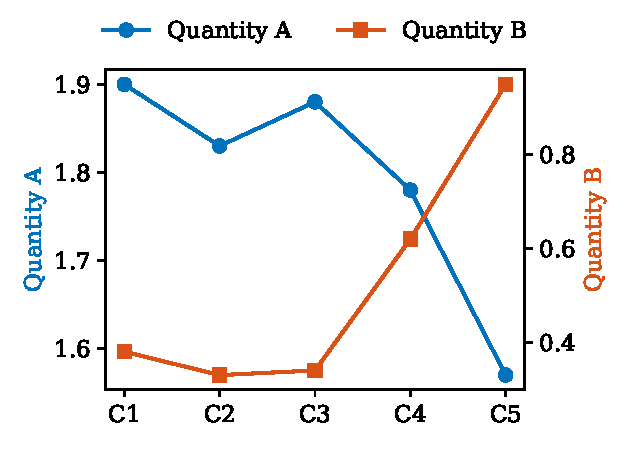
\includegraphics[width=\linewidth]{figures/sample-plot}
        \caption{A vector figure (PDF).}\label{fig:plot}
      \end{figure}
    \end{column}
    \begin{column}{0.48\textwidth}
      \begin{figure}
        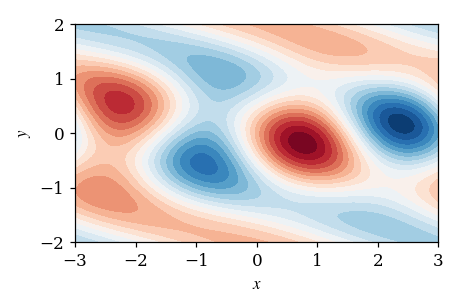
\includegraphics[width=\linewidth]{figures/sample-field}
        \caption{A raster figure (PNG).}\label{fig:field}
      \end{figure}
    \end{column}
  \end{columns}
  \centering Refer to them: Fig.~\ref{fig:plot} and Fig.~\ref{fig:field}.
\end{frame}

% \FigurePlaceholder[width]{height}{text}: a dashed box until the figure exists.
% Caption size for the whole deck: \SetCaptionSize{\footnotesize} (preamble).
\begin{frame}{Placeholders}
  \begin{figure}
    \FigurePlaceholder[0.6\linewidth]{4cm}{\cmd{FigurePlaceholder[0.6\textbackslash linewidth]\{4cm\}\{text\}}}
    \caption{A placeholder keeps the layout while the figure is being made.}
  \end{figure}
\end{frame}

% slideplot: lines from data files (columns by name or number). In the PDF,
% pgfplots draws them; in the HTML deck the plot is interactive: values under
% the pointer, drag to zoom in, double-click to zoom out, click a legend entry
% to hide / show its line. \plotline<2->: a line from step 2 on.
% Options: width, height, xlabel, ylabel, xmin, xmax, ymin, ymax, grid,
% legend; per line x, y, label, color, style, offset (shifts the line along
% x), sep, pdfevery.
\begin{frame}{Plots from data}{interactive in the HTML deck}
  \begin{slideplot}[width=0.9\linewidth, height=5cm, xlabel={Time $t$ (s)},
                    ylabel={Response $y$}]
    \plotline[x=time, y=case1, label={Case 1}]{figures/sample-response.csv}
    \plotline[x=time, y=case2, label={Case 2}]{figures/sample-response.csv}
    \plotline<2->[x=time, y=case3, label={Case 3}, style=dashed]{figures/sample-response.csv}
  \end{slideplot}
\end{frame}

% Panels: \plotpanel[title, xlabel, ylabel] starts a panel, the \plotline
% lines after it are drawn in it. rows / columns lay them out; share=x, y,
% both, none (default: one column -> x, one row -> y, a grid -> both): a
% shared axis has one range and tick labels on the outer panels only, and in
% the HTML deck zooming one panel zooms all. The slideplot's xlabel / ylabel
% are written once; one legend for all panels (one entry per label).
\begin{frame}{Plots in panels}{shared axes, one legend}
  \begin{slideplot}[columns=3, width=0.95\linewidth, height=5cm, xlabel={Time $t$ (s)},
                    ylabel={Response $y$}, legend=outer north]
    \plotpanel[title={Case 1}]
      \plotline[x=time, y=case1, label={Response}]{figures/sample-response.csv}
    \plotpanel[title={Case 2}]
      \plotline[x=time, y=case2, label={Response}]{figures/sample-response.csv}
    \plotpanel<2->[title={Case 3}]
      \plotline[x=time, y=case3, label={Response}]{figures/sample-response.csv}
  \end{slideplot}
\end{frame}
